\section{Der Morse-Komplex und der Raum der gebrochenen Trajektorien}

Wir sind nun bereit, den Morse-Komplex mit Koeffizienten in $\F_2$ (wenigstens) hinzuschreiben.
Wir fixieren für den gesamten Abschnitt eine glatte kompakte Mannigfaltigkeit $M$ und ein
Morse-Smale Paar $(f, X)$, und für jeden kritischen Punkt $p$ von $f$ eine Morse Umgebung 
$(\psi_p, \Omega(p))$, sodass $\psi(\Omega(p)) = U(\eps_p, \eta_p)$ wie in der Notation zu Morse 
Umgebungen~\ref{def: notation morse umgebung}. Dann definiere $C_k (M, (f, X))$ als das $\F_2$ Modul, 
das von den kritischen Punkten von $f$ mit Index $k$ erzeugt wird. Außerdem sei 
$n_X(p, q) = \# \Lt (p, q) \mod 2$. Dann definiere für einen kritischen Wert $p$:
\[ \del_X (p) := \sum_{\substack{ q \in \Crit(f) \\ \Index (p) + 1 = \Index (q) }} n_X(p, q)p . \]

Das Ziel dieses Abschnittes ist es zu zeigen, dass der Komplex $C_{\ast}(M, (f, X))$ wohldefiniert
ist, also dass gilt $n_X (p, q) < \infty$, und dass es ein Kettenkomple ist, also dass 
$\del_X \circ \del_X = 0$. Sobald das gezeigt wurde ist es ein Leichtes, den Komplex auch über die 
ganzen Zahlen zu definieren.

\subsection*{Wohldefiniertheit}

\begin{definition}[Der Raum der gebrochenen Trajektorien]
    \label{def: raum der gebrochenen trajektorien}
    Es seien $p$ und $q$ kritische Punkte von $f$. Der \textit{Raum der gebrochenen Trajektorien} ist
    \[ \Lb (p, q) = 
        \bigcup_{k \in \N} \left( \bigcup_{\substack{c_1, \dots, c_{k - 1} \\ \in \Crit(f)}} 
            \Lt (p, c_1) \times \Lt (c_1, c_2) \times \dots 
                \times \Lt (c_{k - 2}, c_{k - 1}) \times \Lt (c_{k - 1}, q) \right) . \]
\end{definition}

Obwohl die Formulierung recht sperrig wirkt ist sie doch intuitiv: 
$\ell \in \Lt (p, q)$ ist eine \glqq Verbindung\grqq{} zwischen den kritischen Punkten $p$ und $q$ 
entlang des Pseudo-Gradientenfeldes $X$. Ein Element 
$(\ell_1, ..., \ell_k) \in \Lt (p, c_1) \times \dots \times \Lt (c_{k - 1}, q) \subseteq \Lb (p, q)$
ist eine \glqq Verbindung\grqq{} zwischen $p$ und $q$ entlang des Pseudo-Gradientenfeldes $X$, die noch 
bei den kritischen Punkten $c_1, \dots, c_{k - 1}$ \glqq Halt\grqq{} macht. 

Offensichtlich gilt:
\begin{itemize}
    \item Ist $\Index (p) + 1 = \Index (q)$, so ist $\Lb (p, q) = \Lt (p, q)$.
    \item Ist $\Index (p) + 2 = \Index (q)$, so ist 
        $\Lb (p, q) = \Lt (p, q) \cup \bigcup_{c \in \Crit (f)} \Lt(p, c) \times \Lt(c, q)$
\end{itemize}

Wir werden sehen, dass man wie mit der Notation angedeutet $\Lb (p, q)$ mit einer Topologie ausstatten 
kann, sodass es die Kompaktifizierung von $\Lt (p, q)$ ist. (In der Tat ist ja 
$\Lt (p, q) \subseteq \Lb (p, q)$).

\begin{definition}[Topologie von $\Lb (p, q)$]
    Ese seien $p$ und $q$ kritische Punkte von $f$. Wir erinnern uns an unsere Vorstellung von Morse-
    Umgebungen $U = U(\eps, \eta)$ wie in~\ref{def: notation morse umgebung}:
    \begin{itemize}
        \item $\del_+ U$ sind alle Punkte auf dem Rand von $U$, auf denen Trajektorien von $X$ in 
            die Umgebung $U$ eintreten.
        \item $\del_- U$ sind alle Punkte auf dem Rand von $U$, auf denen Trajektorien von $X$ die
            Umgebung $U$ verlassen.
        \item Die Trajektorien von $X$ verlaufen tangential zu $\del_0 U$.
    \end{itemize}
    Es sei nun 
    \[ \ell = (\lambda_1, \dots, \lambda_k) 
        \in \Lt (p, c_1) \times \dots \times \Lt(c_{k - 1}, q) \subseteq \Lb (p, q) . \]
    Seien $U_i = U_i (\eps_i, \eta_i)$ Morse Umgebungen von $c_i$ und $U_0$ und $U_k$ Morse 
    Umgebungen von $p$ und $q$. $\lambda_i \cap \del_+ U_i$ ist der Punkt, an dem $\lambda_i$
    in $U_i$ eintritt, und $\lambda_{i + 1} \cap \del_- U_i$ ist der Punkt, an dem $\lambda_{i + 1}$
    die Umgebung $U_i$ verlässt. Es sei $U_i^-$ eine Umgebung von $\lambda_i \cap \del_+ U_i$ in 
    $\del_+ U$ und $U_i^-$ eine Umgebung von $\lambda_{i + 1} \cap \del_- U_i$ in $\del_- U_i$. 
    Seien dann $U^- = \bigcup U_i^-$ und $U^+ = \bigcup U_i^+$. Dann definiere die Menge 
    $\mathcal{U} (\ell, U^-, U^+)$ wie folgt:

    Wir sagen 
    $\ell' = (\mu_1, ..., \mu_{k'}) \in \Lt (p, c_{i_1}) \times \dots \times \Lt (c_{i_{k'-1}}, q)$
    ist in $\mathcal{U}(\ell, U^-, U^+)$ enthalten, falls $\mu_j \cap U_j^+ \neq \varnothing$
    und $\mu_j \cap U_{j + 1}^- \neq \varnothing$. 
    Dann ist $\mathcal{W} \subseteq \Lb (p, q)$ offen genau dann, wenn es für jedes 
    $\ell \in \mathcal{W}$ Umgebungen $U^+$ und $U^-$ wie oben gibt, sodass 
    $\mathcal{U}(\ell, U^+, U^-) \subseteq \mathcal{W}$.
\end{definition}

\begin{remark}
    Die Topologie von $\Lt(p, q)$ als Quotient stimmt mit der von $\Lb(p, q)$ überein.
    \todo{}
\end{remark}

\begin{prop}
    \label{prop: Lb ist kompakt}
    Es seien $p$ und $q$ kritische Punkte von $f$. Dann ist $\Lb (p, q)$ kompakt.
\end{prop}

Um diese Proposition zu beweisen benötigen wir noch ein Lemma:

\begin{lemma}
    \label{lemma: konvergenz einer folge}
    Es sei $x \in M$ \emph{kein} kritischer Punkt von $f$. Sei außerdem $(x_n)_n$ eine Folge in
    $M$ die gegen $x$ kovnvergiert und seien $y_n$ und $y$ Punkte, die auf den selben Trajektorien
    wie $x_n$ und $x$ liegen. Es gelte außerdem $f(y_n) = f(y)$ für alle $n \in \N$. Dann gilt
    \[ \lim_{n \to + \infty} y_n = y . \]
\end{lemma}

\begin{proof}
    Es sei $U$ eine Umgebung von $\Crit (f)$. Dann ist $\opd f (\cdot) (X)$ nie Null, und ähnlich wie 
    Im Beweis vom ersten Deformationslemma~\ref{satz: erstes deformationslemma} betrachten wir das
    Vektorfeld 
    \[ Y = - \frac{1}{\opd f (\cdot) (X)} \cdot X \]
    Auf $M - U$. Sei $\phi$ die von $Y$ erzeugte 1-Parameter Gruppe aus Diffeomorphismen. 
    Da $Y$ in die selbe Richtung zeigt wie $X$, stimmen die Trajektorien von $Y$ mit denen von $X$ 
    überein und es gilt 
    \[ f(\phi_t(z)) = f(z) - t . \]
    Dann gilt
    \[ \lim_{n \to \infty} y_n 
    = \lim_{n \to \infty} \phi_{- f(y_n) + f(x_n)}(x_n) 
    = \lim_{n \to \infty} \phi_{- f(y) + f(x_n)}(x_n) 
    = \phi_{- f(y) + f(x)}(x) = y \]
\end{proof}

\begin{proof}[Beweis von Proposition~\ref{prop: Lb ist kompakt}]
    Es sei $(\ell_n)_n$ eine Folge in $\Lb (p, q)$. Um zu zeigen, dass $Lb (p, q)$ kompakt ist
    müssen wir zeigen, dass $(l_n)_n$ eine konvergente Teilfolge besitzt.

    Wir nehmen zuerst an, dass für alle $n \in \N$ die Trajektorie $\ell_n$ in $\Lt (p, q)$.
    Seien $U$ und $V$ Morse Umgebungen von $p$ und $q$ in der Form wie bei der eingeführten
    Notation für Morse Umgebungen~\ref{def: notation morse umgebung}.
    Es außerdem sei $\ell_n^- \in M$ der Punkt, an dem $\ell_n$ die Morse Umgebung $U$ verlässt 
    und $\ell_n^- \in M$ der Punkt, an dem $\ell_n$ in die Morse Umgebung $V$ eintritt.
    $\ell_n^-$ und $\ell_n^+$ sind im Schnitt von $\del U$ bzw. $\del V$ und der stabilen bzw. 
    instabilen Mannigfaltigkeit. Diese Schnitte sind Kugeloberflächen, also kompakt. Die Folgen 
    $(l_n^-)_n$ und $(\ell_n^+)_n$ haben also konvergente Teilfolgen, wir können demnach ohne 
    Beschränkung der Allgemeinheit annehmen, dass sie konvergent sind. Setze
    \[ \lim_{n \to \infty} \ell_n^- = p^- \text{ und } \lim_{n \to \infty} \ell_n^+ = q^+ . \]
    Sei $\phi$ die von $X$ erzeugte 1-Parameter Gruppe aus Diffeomorphismen, dann ist 
    $\gamma = \phi_{\bullet}(p^-)$ die Trajektorie von $p^-$. Sei 
    $c = \lim_{n \to \infty} \phi_t(p^-)$. $c$ ist nach 
    Proposition~\ref{prop: trajektorien enden in kritischen punkten} ein kritischer Punkt,
    also ist $\gamma \in \Lt (p, c)$. Es sei nun $W$ eine Morse-Umgebung von $c$, die auch
    die Form hat wie in~\ref{def: notation morse umgebung}. Da $\phi$ glatt ist, muss für $n$ 
    groß genug auch $\ell_n$ die Morse Umgebung $W$ von $c$ kreuzen. Sei $d_n^+ \in M$ der Punkt, an
    dem $\ell_n$ in $W$ eintritt. Dann gilt $d_n^+, d^+ \in \del_+ W$, also gilt $f(d_n^+) = f(d^+)$
    für alle $n$. Da $d_n^+$ auf der selben trajektorie wie $p_n^-$ liegt, und $d^+$ auf der selben 
    Trajekorie wie $p^-$,folgt da $\lim p_n^- = p^-$ mit dem letzten 
    Lemma~\ref{lemma: konvergenz einer folge}: 
    \[ \lim_{n \to \infty} d_n^+ = d^+ . \]
    Falls $c = q$, dann ist $\lim \ell_n = \gamma \in \Lt (p, q) \subseteq \Lb (p, q)$, also hat 
    dann die Folge $(\ell_n)_n$ eine konvergente Teilfolge. Es sei also $c \neq q$. Dann muss 
    $\ell_n$ die Morse Umgebung $W$ wieder durch einen Punkt $d_n^-$ verlassen. Wie oben können wir 
    ohne Beschränkung der Allgemeinheit annehmen, dass die Folge $(d_n^-)_n$ konvergent ist, da
    sie zumindest eine konvergente Teilfolge besitzt. Wir definieren dann $d^- = \lim d_n^-$. 
    $d^-$ liegt in der instabielen Mannigfaltigkeit von $c$, denn wäre dies nicht der Fall, dann 
    führt das zu einem Widerspruch:
    
    Angenommen $d^- \notin \unst (c)$. Dann wäre $d^-$ auf der Trajektorie von einem Punkt
    $d^+_{\ast} \in \del_+ W$, der nicht in $\stab (c)$ enthalten ist. Wieder wegen des vorherigen
    Lemmas~\ref{lemma: konvergenz einer folge} ist dann $\lim d_n^+ = d^+_{\ast}$, also gilt dann
    $d^+ = d^+_{\ast}$, aber es gilt $d^+ \in \stab{c}$.
    
    Wir können nun wieder mit dem selben Argument zeigen, dass dann die Trajektorie von $d^-$ im
    kritischen Punkt $q$ endet, also liegt dann $\lim \ell_n$ in $\Lt (p, c) \times \Lt (c, q)$.

    Jetzt fehlt uns noch der allgemeine Fall. Wir müssen also für eine Folge $(\ell_n)_n$ in 
    $\Lb (p, q)$ zeine konvergente Teilfolge finden. Wegen der Glattheit von $\phi$ können wir annehmen,
    dass für $n$ groß genug alle $\ell_n$ die Form 
    \[ \ell_n = (\ell^1_n, \dots, \ell^k_n) \in \Lt (p, c_1) \times \dots \times \Lt (c_{k - 1}, q) \]
    haben. Wir finden mit der vorheringen Überlegung komponentenweise eine Teilfolge, sodass wir 
    für den grenzwert maximal noch $k - 1$ kritische Punkte als \glqq Zwischenstopp\grqq{} einfügen
    müssen. 
\end{proof}

\begin{remark}
    Sind nun $p$ und $q$ kritische Punkte von $f$ mit $\Index (p) = \Index (q) + 1$, dann ist 
    $\Lt(p, q)$ $0$-dimensionale Mannigfaltigkeit. Außerdem ist $\Lt (p, q)$ eine Abgeschlossene
    Teilmenge von $\Lb (p, q)$, und wie wir in der letzten Proposition~\ref{prop: Lb ist kompakt}
    gezeigt haben, ist $\Lb(p, q)$ kompakt, also auch $\Lt(p, q)$, also ist $\Lt (p, q)$ endlich.
    Damit ist schon mal $n_X (p, q)$ wohldefiniert.
\end{remark}

\subsection*{Der Morse Komplex ist ein Kettenkomplex}

Wir wollen zeigen, dass der Morse-Komplex tatsächlich ein Kettenkomplex ist, also dass $\del^2 = 0$.
Dafür genügt es zu zeigen, dass für einen kritischen Punkt $p$ mit Index $k + 1$ gilt $\del^2 (0) = 0$, 
also dass für jeden weiteren kritischen Punkt mit Index $k + 1$ gilt, dass die Zahl
$\# (\Lb (p, q) - \Lt (p, q))$ gerade ist. Wir benutzen die folgende Aussage, ohne sie zu beweisen:

\begin{theorem}[Klassifizierung kompakter 1-Mannigfaltigkeiten]
    \label{satz: klassifizierung kompakter 1-mannigfaltigkeiten}
    Es sei $M$ eine kompakte zusammenhängende Mannigfaltigkeit mit Rand. Dann ist
    \begin{itemize}
        \item $M$ diffeomorph zu $S^1$, falls $\del M = \varnothing$
        \item $M$ diffeomorph zu $[0, 1]$, falls $\del M \neq \varnothing$
    \end{itemize}
\end{theorem}

% \begin{proof}
%     Betrachte zuerst den ersten Fall, also dass $M$ keinen Rand hat. Es sei 
%     $\{ (U_1, \phi_1), \dots, (U_n, \phi_n) \}$ ein Atlas von $M$. Ohne Beschränkung der 
%     Allgemeinheit können wir annehmen, dass alle $U_i$ zusammenhängend sind. 
%     Da $M$ zusammenhängend ist, können wir außerdem annehmen, dass 
%     $\bigcup_{i = 1}^k U_i$ für alle $k$ zusammenhängend ist. Dann existiert ein $1 \leq k < n$, 
%     sodass $\bigcup_{i = 1}^k U_i$ diffeomorph zu $\R$ ist, aber $\bigcup_{i = 1}^{k + 1} U_i$ 
%     nicht. Setze $U := \bigcup_{i = 1}^k U_i$ und $V = U_{k + 1}$. Seien $\phi \colon U \to \R$
%     und $\psi \colon V \to \R$ Diffeomorphismen. 
%     \begin{claim*}
%         Ist $M = U \cup V$ eine 1-dimensionale Mannigfaltigkeit, $U$ und $V$ diffeomorph zu 
%         $\R$, dann ist $M$ diffeomorph zu $S^1$ oder $\R$.
%     \end{claim*}

%     \begin{smallproof}
%         Ohne Beschränkung der Allgemeinheit ist $U \not\subseteq V$ und \\ 
%         $V \not\subseteq U$. Dann gibt es zwei Möglichkeiten:
%         \begin{itemize}
%             \item $\phi(U \cap V)$ und $\psi(U \cap V)$ sind offene Halbintervalle
%             \item $\phi(U \cap V)$ und $\psi(U \cap V)$ sind jeweils die disjunkte Vereinigung
%                 zweier offener Halbintervalle
%         \end{itemize}
%         Im ersten Fall ist $M$ homeomorph zu $\R$:

%         Wir dürfen annehmen, dass $\phi(U \cap V) = (- \infty, a)$ und $\psi(U \cap V) = (b, \infty)$,
%         ansonsten ersetze $\phi$ mit $\-phi$ bzw. $\psi$ mit $-\psi$. Die Verkettung
%         \[ \begin{tikzcd}
%             (- \infty, a) = \phi(U \cap V) \arrow[r, "\phi^{-1}"] & 
%                 U \cap V \arrow[r, "\psi"] & 
%                 \psi(U \cap V) = (b, \infty)
%         \end{tikzcd} \] 
        
%         Ist insbesondere injektiv, also auch monoton wachsend. 
%         \todo{}
%     \end{smallproof}
% \end{proof}

\begin{prop}
    \label{prop: gebrochene trajektorien sind 1-dim mannigfaltigkeit}
    Es seiein $p$ und $q$ kritische Punkte von $f$ mit $\Index (p) = k + 1$ und $\Index (q) = k - 1$
    für ein $k \in \N_0$. Dann ist $\Lb (p, q)$ eine 1-dimensionale Mannigfaltigkeit mit Rand, und das
    Innere von $\Lb (p, q)$ ist $\Lt (p, q)$.
\end{prop}

Mit dieser Proposition folgt dann mit der Kalssifizierung von $1$-Mannigfaltigkeiten mit 
Rand~\ref{satz: klassifizierung kompakter 1-mannigfaltigkeiten} schon, dass der Morse Komplex ein
Kettenkomplex ist.

\begin{bigproof}
    Wir wissen schon, dass $\Lt (p, q) \subseteq \Lb(p, q)$ eine $1$-dimensionale Mannigfaltigkeit ist. 
    Um sagen zu können, dass $\Lb (p, q)$ eine $1$-dimensionale Mannigfaltigkeit mit Rand ist, und 
    insbsondere, dass $\Lb (p, q)$ das Innere von $\Lt(p, q)$ ist, reicht die folgende Aussage über 
    $\Lb(p, q)$:
    Es sei $c$ ein weiterer kritischer Punkt mit Index $k$.
    Sei $\lambda_1 \in \Lt (p, c)$ und $\lambda_2 \in \Lt (c, q)$. Dann existiert eine offene Umgebung
    $U \subseteq \Lb (p, q)$ von $(\lambda_1, \lambda_2)$, ein $\delta > 0$ und ein Homeomorphismus
    $\psi \colon [0, \delta) \to U$, sodass gelten: 
    \begin{enumerate}
        \item $\psi|_{(0, \delta)}$ ist glatt.
        \item $\psi(0) = (\lambda_1, \lambda_2)$.
        \item $\psi((0, \delta)) \subseteq \Lt (p, q)$.
        \item Für jede Folge $(\ell_n)_n$ in $\Lt (p, q)$ die gegen $(\lambda_1, \lambda_2)$ konvergiert 
            gilt $\ell_n \in \Ima \psi$ für $n$ groß genug.
    \end{enumerate} 
    Die letzten beiden Bedingungen stellen sicher, dass $\Lt (p, q)$ tatsächlich das Innere von 
    $\Lb (p, q)$ ist.
    Wir begeben uns also auf die (recht lange) Suche nach einer solchen Abbildung $\psi$. 

    Wir machen ein Paar Konstruktionen. Sei $\alpha := f(c)$ und $(V, \psi)$ eine Morse Umgebung von
    $c$, $\eps$, $\eta$ und $\Omega(c)$ wie in der Notation zu Morse 
    Umgebungen~\ref{def: notation morse umgebung}. Dann sind 
    $f(\del_+ \Omega) = \alpha + \eps$ und $f(\del_- \Omega) = \alpha - \eps$ für ein $\eps > 0$.
    Außerdem gilt, wie schon vorher, dass 
    \begin{align*}
        S_+ (c) := & \stab (c) \cap f^{-1}(\alpha + \eps) \isom S^{n - k - 1} \\
        S_- (c) := & \unst (c) \cap f^{-1}(\alpha - \eps) \isom S^{k - 1} .
    \end{align*}
    Es sei $a_1 \in M$ der Punkt, an dem $\lambda_1$ auf $\Omega(c)$ trifft, also 
    $a_1 = S_+ (c) \cap \lambda_1$, und $a_2$ der Punkt, an dem $\lambda_2$ die Umgebung $\Omega (c)$ 
    wieder verlässt, also $a_2 = S_- (c) \cap \lambda_2$. $\alpha + \eps$ ist kein kritischer Wert 
    von $f$ und es gilt $f^{-1}(\alpha + \eps) \pitchfork \unst (p)$, also ist mit 
    Proposition~\ref{prop: schnitt von transversalen untermannigfaltigkeiten} 
    $P = f^{-1}(\alpha) \cap \unst (p)$ eine Mannigfaltigkeit mit Dimension $(n - 1) + (k + 1) - n = k$.
    Da $X$ die Smale-Eigenschaft erfüllt gilt 
    $\unst (p) \supseteq P \pitchfork S_+ (c) \subseteq \stab(c)$, also ist $P \cap S_+ (c)$
    mit Proposition~\ref{prop: schnitt von transversalen untermannigfaltigkeiten} eine 
    Untermannigfaltigkeit der Dimenion $(k) + (n - k) - n = 0$. Offensichtlich gilt 
    $a_1 \in P \cap S_+ (c)$. Es sei $D^k_{\eps} = \{ x \in \R^k : \| x \| < \eps \}$. Dann existiert 
    eine Umgebung D von $a_1$ und ein Diffeomorphismus $\Psi : D \longto D^k_{\delta}$ mit 
    $\Psi(a_1) = 0$, sodass $P \supseteq D \cap S_+ (c) = a_1$ und $D \subseteq \del_+ \Omega (c)$.
    Wir versuchen die Kernidee des Beweises zu verstehen:

    \begin{figure}
        \centering
        \begin{minipage}{.5\textwidth}
          \centering
          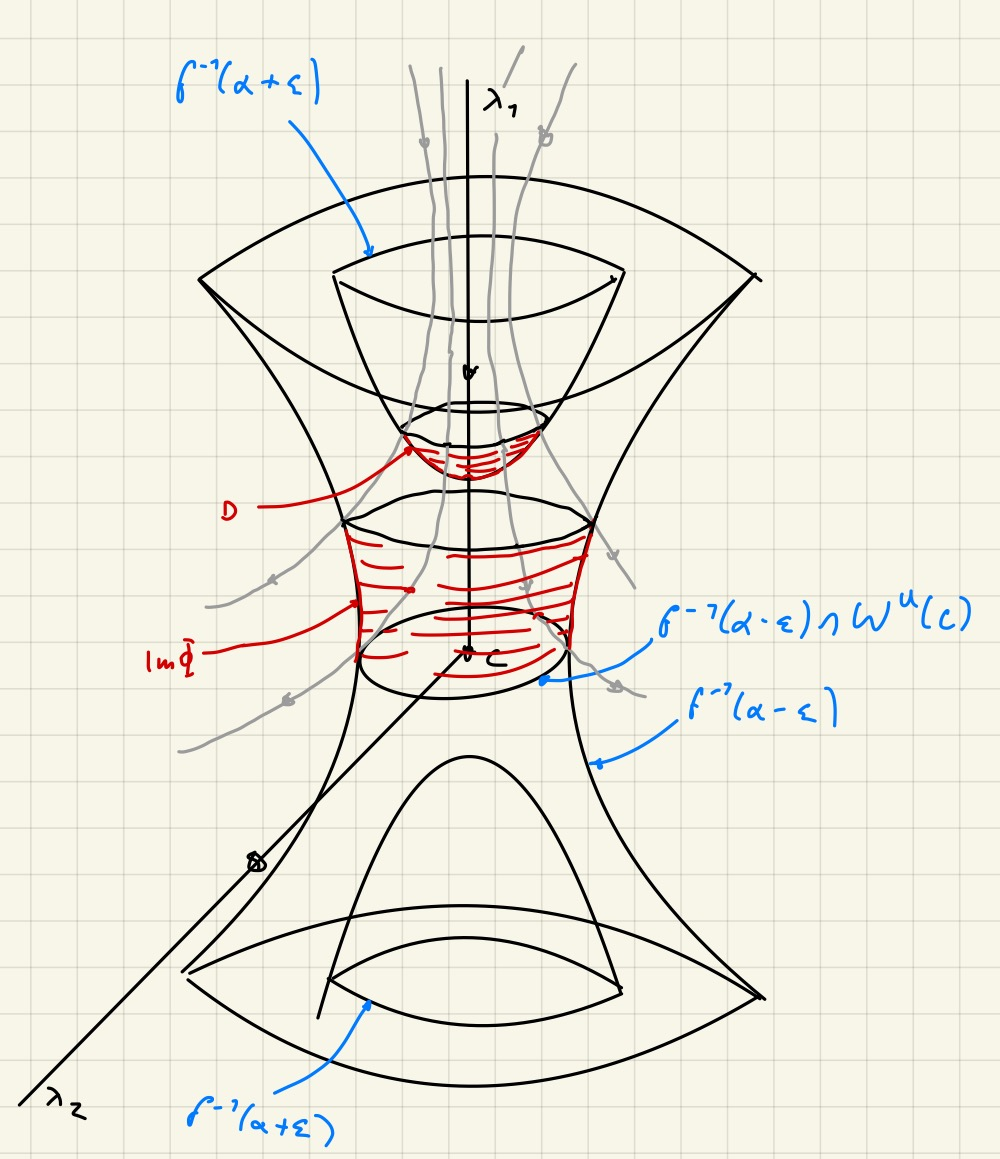
\includegraphics[width=.85\linewidth]{../resources/bew-gebrochene-trajektorien-sind-1-dim-mannigfaltigkeit-1.JPG}
          \captionof{figure}{A figure}
          \label{fig: test1}
        \end{minipage}%
        \begin{minipage}{.5\textwidth}
          \centering
          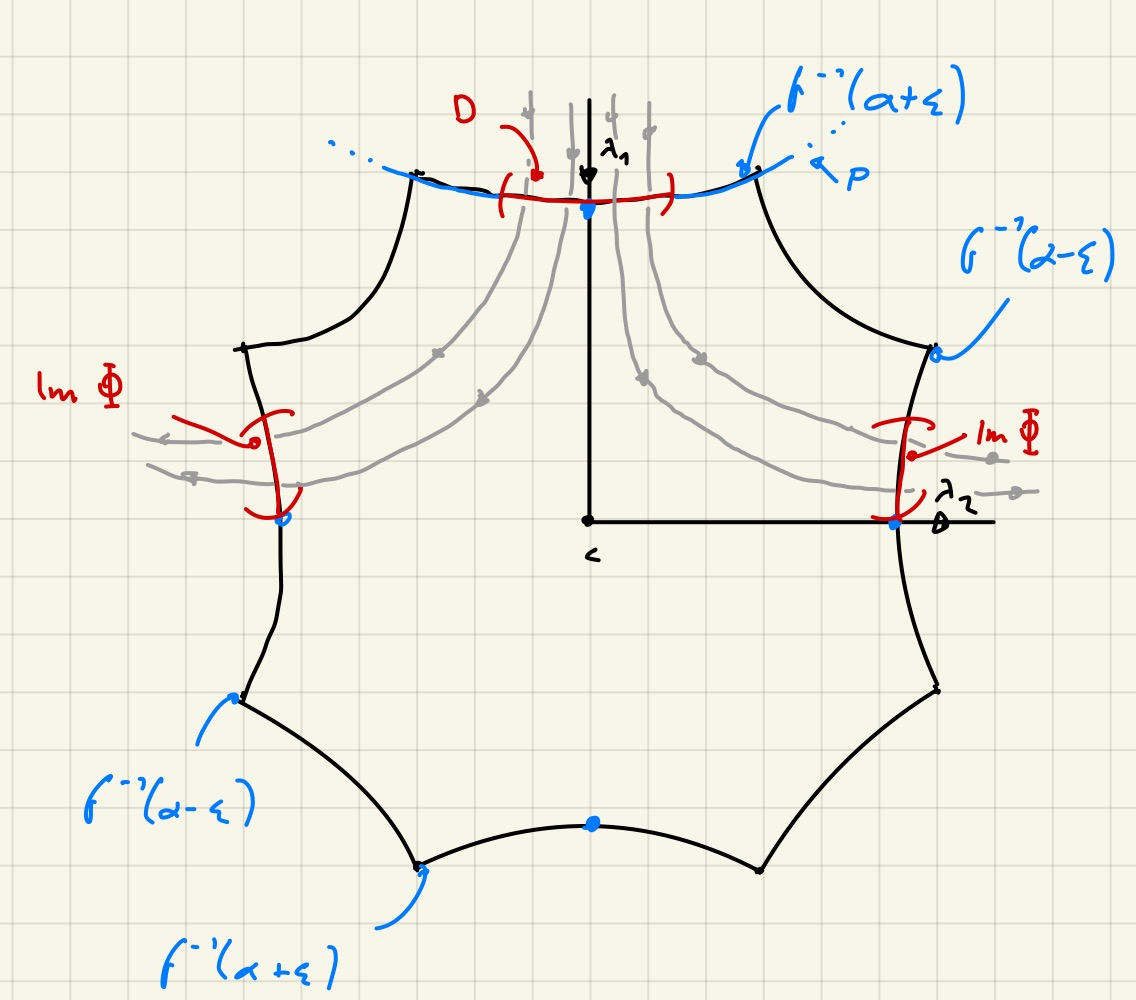
\includegraphics[width=.85\linewidth]{../resources/bew-gebrochene-trajektorien-sind-1-dim-mannigfaltigkeit-2.JPG}
          \captionof{figure}{Another figure}
          \label{fig: test2}
        \end{minipage}
    \end{figure}

    Man betrachte die Abbildungen~\ref{fig: test1} und~\ref{fig: test2}.

    Wir versuchen, Menge $D - a_1$ entlang der Trajektorien von $X$ auf den Teil des Randes der Morse 
    Umgebung, an denen die Trajektorien austreten, via einer Abbildung $\Phi$ zu projizieren. Wir werden
    sehen, dass $Q = \Phi \cup S_+(c)$ eine Mannigfaltigkeit mit Rand ist, und dass $\stab (q)$ eine 
    $1-dimensionale Mannigfaltigkeit$ ist. Fügen wir dieser Mannigfaltigkeit den Punkt $a_2$ hinzu, dann
    können wir eine Umgebung von $(\lambda_1, \lambda_2)$ auf die gewünschte Art über die entstandene
    1-dimensionale Mannigfaltigkeit mit Rand parametrisieren. Also:

    \begin{claim}
        Es sei $\phi$ die von $X$ erzeugfte 1-Parameter Gruppe aus Diffeomorphismen. Für jedes 
        $x \in D - a_1$ existiert ein $t_x \in \R$, sodass $\phi_{t_x} (x) \in \del_- \Omega (c)$
        und $x \mapsto t_x$ glatt ist.
    \end{claim}

    \begin{smallproof}
        Via unserer anfangs gewählten Morse Karte $(V, \psi)$, und da wir ohne Einschränkungen $D$ 
        klein genug wählen können, sodass $\psi(D) \subseteq V$, können wir annehmen, dass sich alles im 
        $\R^n$ abspielt ; Sei also ohne Beschränkung $f(x_-, x_+) = - \|x_-\| + \|x_+\|$. Dann ist 
        $\phi$ gegeben durch 
        \[ \phi_t(x_-, x_+) = (e^{2t}x_-, e^{-2t}x_+) . \]
        Falls $(x_-, x_+) \in \del_+ U$ und $x_- \neq 0$, dann gilt auch $x_+ \neq 0$. Setze
        \[ t_{(x_-, x_+)} = \frac{1}{2} \ln \left( \frac{\| x_+ \|}{\| x_- \|} \right) . \]
        Dann gilt
        \[ \phi_{t_{(x_-, x_+)}} (x) = 
            \left( \frac{\| x_+ \|}{\| x_- \|} x_-, \frac{\| x_- \|}{\| x_+ \|} x_+ \right) . \]
        Die Zuordnung $(x_-, x_+) \mapsto t_{(x_-, x_+)}$ ist glatt und 
        \begin{align*}
            f(\phi_{t_{(x_-, x_+)}})(x_-, x_+) = & - \| \frac{\| x_+ \|}{\| x_- \|} x_- \|
                +  \| \frac{\| x_- \|}{\| x_+ \|} x_+ \| \\
                = & - \| x_+ \| + \| x_- \| \\
                = & - \eps .
        \end{align*}
        Es folgt $\phi_{t_{(x_-, x_+)}} (x) \in \del_- U$.
    \end{smallproof}

    Wir haben nun also eine Einbettung $\Phi$ von $D - a_1$ entlang der Trajektorien von $X$ gefunden.
    Wie am Anfang besprochen wollen wir jetzt zeigen:

    \begin{claim}
        Ist $\delta$ klein genug, dann ist $Q = \Phi (D - a_1) \cup S_(c)$ eine $k$ dimensionale 
        Mannigfaltigkeit mit Rand, und es gilt $\del Q = S_- (c)$.
    \end{claim}

    \begin{smallproof}
        Wider spielt sich alles via $\psi$ im $\R^n$ ab.
        Man betrachte die Projektion
        \[ \pi \colon \R^k \times \R^{n - k} ; \pi (x_-, x_+) = x_- . \]
        und ihre Einschränkung $\del_+U \to D_{\delta}^k$
        \todo{weiß net ob das stimmt, naja} Da $S_+ := \psi(\S_+(c)) = (\pi|_{\del_+U})^{-1}(0)$
        und $D \pitchfork S_+$, ist $0$ ein regulärer Wert von $\pi|_{\del_+U}$.
        Also ist $\opd \pi|_{\del_+U} (0)$ surjektiv, und da dim $\del_+U = k = \dim D^k_{\delta}$ ist
        das Differential auch invertierbar. Jetzt können wir den Satz über die Umkehrfunktion anwenden 
        bekommen lokal ein Inverses der Abbildung $\pi|_{\del_+U}$. Es existiert also ein 
        $\delta' \leq \delta$, sodass das inverse von $\pi|_{\del_+U}$ auf $D^k_{\delta'}$ definiert ist.
        Dann ist 
        \begin{align*}
            (\pi|_{del_+U})^{-1} \colon D^k_{\delta'} \longto & D \\
            x_- \longmapsto & (x_-, x_+) =: (x_-m h(x_-))
        \end{align*}
        ein Diffeomorphismus. Da $D \subseteq \del_+U \subseteq f^{-1}(\eps)$, gilt dann 
        $\| h(x_-) \|^2 = \| x_- \|^2 + \eps $. Ist dann 
        $g = \cfrac{h}{\| h \|} \colon D^k_{\delta'} \to S^{n - k - 1}$, dann gilt
        \[ D = \{ (x_-, h(x_-)): x \in D^k_{\delta'} \} 
            = \{ (x_-, \sqrt{\| x_- \|^2 + \eps} \cdot g(x_-)): x \in D^k_{\delta'} \} . \]
        Dann bekommen wir mit der Einbettung aus Behauptung 1 und da $\| g(x_-) \| = 1$:
        \[ \Phi(D - a_1) = 
            \left\{ \left( \frac{\sqrt{\| x_- \|^2 + \eps}}{\| x_- \|} \, x_-, \; 
                    \| x_- \| \, g(x_-) \right) : 
                x_- \in D^k_{\delta'} - 0 \right\} \]
        Wir können nun auf $D^k_{\delta'}$ Polarkoordinaten anwenden. wir erhalten einen Diffeomorphismus
        \begin{align*}
            H = \Phi \circ \rho \colon (0, \delta') \times S^{k-1} \longto & D \subseteq \del_-U \\
            (r, v) \longmapsto & ( \sqrt{r^2 + \eps} \cdot v, r \cdot g(\rho(r, v)))
        \end{align*}
        $g$ ist auf ganz $D^k_{\delta'}$ definiert, und wenigstens in einer Umgebung von $0$ beschränkt.
        Also können wir $H$ stetig in $0$ durch
        \[ H(0, v) = (\sqrt{\eps} \cdot v, \, 0) \]
        fortsetzen. Dann ist $H$ auch weiterhin eine (topologische) Einbettung 
        \[ H \colon [0, \delta') \times S^{k - 1} \longto \Phi(D - a_1) \cup S_- , \]
        und es gilt 
        \[ H(0, S^{k - 1}) = S_- . \]
    \end{smallproof}
\end{bigproof}

\subsection*{Der Morse Komplex über \texorpdfstring{$\Z$}{TEXT}}

\begin{definition}[Orientierung und Co-Orientierung von Mannigfaltigkeiten]
    Es sei $V$ ein (endlich dimensionaler) Vektorraum. Seien dann $\B_1$ und $\B_2$ zwei Basen von $V$.
    Wir sagen $\B_1$ und $\B_2$ induzieren dieselbe Orientierung, wenn 
    \[ \det \, _{\B_2}[\id_V]_{B_1} > 0 . \]
    \textit{Dieselbe Orientierung induzieren} ist eine Äquivalenzrelation. Eine Orientierung eines 
    Vektorraums ist eine Wahl einer Äquuivalenzklasse.

    Ein \textit{orientierter Atlas} einer $n$-dimensionalen Mannigfaltigkeit $M$ ist ein Atlas 
    $\mathcal{A}$ von $M$, sodass für alle Karten $(U, \phi)$ und $(V, \psi)$ in $\mathcal{A}$ 
    und alle Punkte $p \in M$ gilt
    \[ \det d \psi \circ \phi^{-1} (p) > 0 \]
    Eine \textit{Orientierung} einer Mannigfaltigkeit ist eine Auswahl eines maximalen orientierten Atlas.
    Eine Mannigfaltigkeit heißt orientierbar, falls eine Orientierung für die Mannigfaltigkeit existiert.
\end{definition}

\begin{remark}
    Man kann zeigen, dass es für jeden Vektorraum und jede Mannigfaltigkeit genau zwei Orientierungen
    gibt. Man sagt die ausgewählte Orientierung ist \textit{positiv} und die andere \textit{negativ}.
\end{remark}

Wir haben nun den Morse Komplex über $\F_2$ definiert. Wir wollen noch allgemeiner einen Komplex
über $\Z$ definieren. Die meiste Arbeit dafür ist nun schon gemacht. 
Wir können die Morse Umgebungen jedes kritischen Punktes orientieren. Sind $p$ und $q$ 
kritische Punkte mit $\Index (p) = \Index(q) + 1$, dann ist 
$\mathcal{W} (p, q) = \unst (p) \cap \unst (q)$ eine $1$-dimensionale kreisscheibe, also 
orientierbar. 
